\section{EDO's de 1\textordfeminine ordem}


\begin{frame}
\frametitle{ EDO's de 1\textordfeminine ordem}
%\begin{scriptsize}

\uncover<1->{Uma EDO de $1^{\underline{a}}$ ordem é uma equação da forma
$$F(t,y,y')=0.$$ 
Um problema da forma
$$\left\{\begin{array}{l}
F(t,y,y')=0\\
y(t_0)=y_0
\end{array}\right.$$
é dito \dt{problema de valor inicial (PVI)}. Uma \dt{solução geral} de uma EDO de $1^{\underline{a}}$ ordem, é uma família de soluções que dependem de uma constante arbitrária, tal que toda solução particular pode ser obtida desta família por uma escolha apropriada da constante.}

%\uncover<2->{\begin{exe}
%Encontre a solução geral da equação $\frac{dy}{dt}=e^{3t}$ e uma solução do PVI
%$$\left\{\begin{array}{l}
%\dps\frac{dy}{dt}=e^{3t}\\
%\\
%y(1/3)=e/3.
%\end{array}\right.$$
%\end{exe} }

%\end{scriptsize}
\end{frame}


\begin{frame}{ }
	
	\begin{exampleblock}{Modelo Populacional Malthusiano}
		Este tipo de modelo é razoável para descrever populações que tem {\color{cyan}recurso ilimitados para crescimento e ausência de predadores}. 
		\begin{itemize}
			\item {\color{blue}$y(t)$}: número de indivíduos de uma população no instante $t$.
			\item {\color{red}$y'(t)$}: taxa de crescimento de uma população no instante $t$.
			
			\item Supõe-se que a {\color{red} taxa de crescimento} de uma população é proporcional à {\color{blue} população presente} 
			\[{\color{red}y'(t)}=k{\color{blue}y(t)}\]
		\end{itemize}
		
		
		\medskip
		
		Supondo que a população no instante $t=0$ é $y_0$, determine a função $y=y(t)$. Em quanto tempo a população dobra de tamanho?
	\end{exampleblock}
\end{frame}



\begin{frame}
\begin{casa}
\begin{enumerate}
\item Determine uma solução geral para a equação
\[y'(t)=y(t).\]

\item Determine uma solução para o PVI
\begin{equation*}
\begin{cases}
y'=y\\
y(0)=2
\end{cases}
\end{equation*}
\end{enumerate}



\end{casa}
\end{frame}

\begin{frame}{Campos de Direções}
\dt{Campos de Direções} são ferramentas validas no estudo de soluções de equações diferenciais da forma
\[y'(t)=f(t,y),\]
onde $f$ é uma função dada chamada de \dt{função taxa de variação}. Ele é construído desenhando-se em cada ponto de uma malha retangular um segmento de reta  cujo coeficiente angular é valor de $f$ naquele ponto.


\end{frame}

\begin{frame}
\begin{exe}
Campo de direções de $y'=y$
\begin{center}
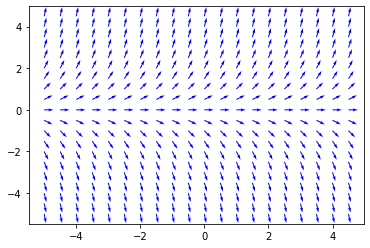
\includegraphics[scale=0.7]{CD-1.png}
\end{center}
\end{exe}
\end{frame}



\begin{frame}
\frametitle{Equações Separáveis }
%\begin{scriptsize}

\uncover<1->{As EDO's de 1\fm ordem \dt{separáveis} são equções da forma
$$g(y)\frac{dy}{dx}=f(x).$$
Integrando esta equação em relação a $x$ temos que
$$\int g(y)y'dx=\int f(x)dx+C.$$
Fazendo a substituição $u=y(x)$, $du=y'(x)dx$ temos que
$$\int g(u)du=\int f(x)dx+C.$$
Assim, se $G$ é uma primitiva de $g$ temos que 
$$G(y(x))=\int f(x) dx +C$$ }
%\end{scriptsize}
\end{frame}


\begin{frame}{Crescimento Populacional Logístico}
	Vimos que um modelo simples de crescimento populacional é aquele em que se supõe que a taxa de crescimento de uma população \textcolor{blue}{$\frac{dy}{dt}$} é proporcional à população presente \textcolor{blue}{$y(t)$} naquele instante.	O \dt{crescimento logístico}, leva em conta que a população tem um valor máximo sustentável \textcolor{red}{$M$}. Quando a população se aproxima da capacidade máxima, os recursos tornam-se menos abundantes e a taxa de crescimento começa a diminuir. Uma relação simples  que exibe esse comportamento é quando 
	\[\textcolor{blue}{\frac{dy}{dt}}={\color{orange}k}\textcolor{blue}{y}(\textcolor{red}{M}-\textcolor{blue}{y}) \]
	
	%\begin{exe} Biólogos colocaram em um lago 400 peixes e estimaram a capacidade de suporte como 10.000. O número de peixes triplicou no primeiro ano. Encontre uma expressão para o tamanho da população de peixes depois de $t$ anos.
	%\end{exe}	
	%	Usando-se o método de frações parciais, pode-se mostrar que a população é modelada por:
	%	\[{\color{blue}y(t)}=\frac{{\color{red}M}}{1+Ce^{-{\color{orange}k}{\color{red}M}t}},\ t\geq 0.\]
	%	
	
\end{frame}

\begin{frame}{ }


%\begin{minipage}{0.55\textwidth}
\begin{exe}
Considere o problema de crescimento logístico:
	\[\begin{cases}
y'=y(1-y)\\
y(0)=y_0, y_0\geq 0.
\end{cases}
\]
Mostre que a solução geral é dada por:
\[y(t)=\frac{1}{1+Ce^{-t}}, t\in \R.\]
\end{exe}
%\end{minipage}
%\begin{minipage}[c]{0.4\textwidth}
%\begin{figure}
%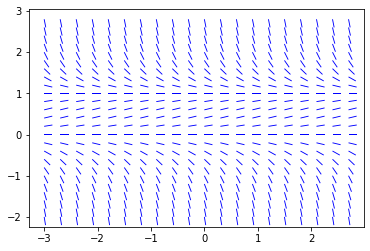
\includegraphics[scale=0.5]{CD-logistico.png}
%\caption{Campo de direções}
%\end{figure}
%\end{minipage}


\end{frame}

\begin{frame}
\begin{block}{Solução geral}
\[y(t)=\frac{1}{1+Ce^{-t}}, t\in \R.\]
\end{block}
\begin{figure}
\centering
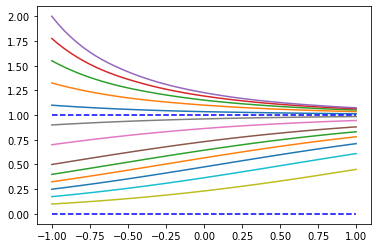
\includegraphics[scale=0.65]{sol-logistico-capa.png}
\caption{Família de Soluções para diversos valores de $C$.}
\end{figure}
\end{frame}


\begin{frame}

\begin{exe}
\[y'=\frac{x^2}{1-y^2}\]
\end{exe}

Solução geral
\[y^3+x^3-3y=C\]

\begin{figure}
\centering
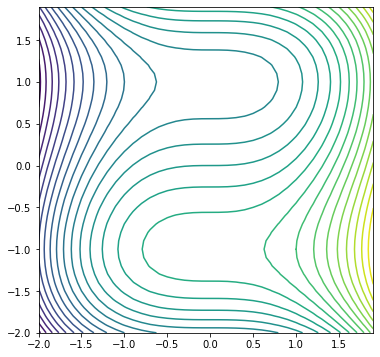
\includegraphics[scale=0.35]{sol-ex-sep.png}
\caption{Família de Soluções para diversos valores de $C$.}
\end{figure}

\end{frame}


\begin{frame}
\frametitle{EDO's Lineares de 1\fm ordem }
%\begin{scriptsize}

As \dt{EDO's lineares de 1\fm ordem} são equações que podem ser escritas da forma
\[\frac{dy}{dt}+{\color{cyan} p(t)}y={\color{cyan} q(t)}.\]

\begin{block}{Técnina do Fator Integrante}
Multiplicamos a equação por {\color{red} fator integrante} função {\color{red} $\mu(t)$ }
\[{\color{red} \mu(t)} y'(t)+\only<1>{{\color{red}\mu(t)} {\color{cyan} p(t)}y}\only<2->{\underbrace{{\color{red}\mu(t)} {\color{cyan} p(t)}}_{{\color{red} \mu'(t) }}y}={\color{red}\mu(t)}{\color{cyan}q(t)}.\]

\uncover<2->{\[\Rightarrow ({\color{red} \mu(t) }y(t))'={\color{red} \mu(t) }{\color{cyan}q(t)}\]
Que pode ser resolvida por integração direta. O {\color{red} fator integrante} ${\color{red} \mu(t) }$ pode ser obtido por
\[{\color{red} \mu(t) }=e^{\int{\color{cyan} p(t)}dt}.\]
}

\end{block}


 
%\uncover<1->{\begin{exe} Obtenha a solução geral da equação
%$\dps y'+\frac{2}{t}y=t$ e esboce um gráfico com as soluções.  
%\end{exe}}


%\end{scriptsize}
\end{frame}



\begin{frame}
\begin{exe}
Determine a solução gerla da equação diferencial
\[y'+\frac{1}{2}y=\frac{1}{2}e^{t/3}.\]
Encontre a solução particular que passa pelo ponto $(0,1)$.
\end{exe}


\begin{center}
\only<1>{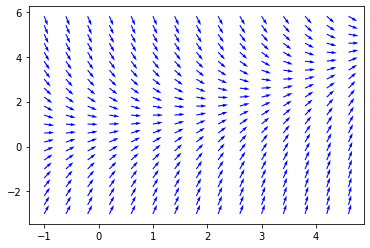
\includegraphics[scale=0.6]{CD-2.png}}
\only<2>{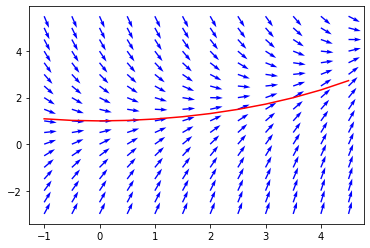
\includegraphics[scale=0.6]{CD-3.png}}
\end{center}

\end{frame}

%\begin{frame}{Queda Livre com Resistência do ar}
%	Sejam um corpo de massa {\color{blue} $m$} que está caindo e que sofre uma força de resistência do ar que é proporcional à velocidade do corpo. Adotando-se o referencial positivo para baixo, a velocidade satisfaz a equação:
%	\[mv'+kv=mg\]
%	
%\end{frame}
\begin{frame}{Queda Livre com Resistência do ar}
	Sejam um corpo de massa {\color{blue} $m$} que está caindo e que sofre uma {\color{red}força de resistência do ar que é proporcional à velocidade do corpo}. Adotando-se o referencial positivo para baixo, a velocidade satisfaz a equação:
\[{\color{blue}m}v'+{\color{red}k}v={\color{blue}m}g\]
	
\begin{exe} Um pára-quedista com o seu pára-quedas pesam 70 quilogramas e salta de uma altura de 1400 metros. O pára-quedas abre automaticamente após 5 segundos de queda. Sabe-se que a velocidade limite é de 5 $m/s$. Determine a velocidade que o pára-quedista atinge no momento que o pára-quedas abre. Quanto tempo demora para a velocidade chegar a 5,1 $m/s$. Como varia a altura em função do tempo?
\end{exe}
\end{frame}

\begin{frame}
\begin{casa}
\begin{enumerate}
\item Determine a solução geral da EDO: $y'-2y=4-t$

\item Resolva o PVI 
\[\begin{cases}
ty'+2y=4t^2\\
y(1)=2.
\end{cases}\]

\item Determine uma fórmula geral para as soluções da EDO: $y'+ay=g(t)$, onde $a$ é uma constante.
\end{enumerate}
\end{casa}
\end{frame}




%\begin{frame}
%\frametitle{ }
%
%
%\uncover<1->{\begin{exe} Encontre a solução do PVI
%$$\left\{\begin{array}{l}
%\frac{dy}{dx}=\frac{2x-1}{3y^2-3}\\
%y(1)=0
%\end{array} \right.$$
%\begin{enumerate}
%\item Determine o \dt{intervalo de validade da solução}, ou seja, o maior intervalo contendo $x_0=1$ para o qual a solução $y(x)$ e sua derivada estão definidas.
%
%\item Determine os pontos onde a solução tem um máximo local.
%
%\item Faça um esboço do gráfico da solução.
%\end{enumerate}
%\end{exe} }
%
%\end{frame}




\begin{frame}
\frametitle{ Equações Exatas}
%\begin{scriptsize}

Uma EDO de 1\fm\ ordem 
\[{\color{red}M(x,y)}+{\color{blue}N(x,y)}\frac{dy}{dx}=0,\]
é dita \dt{equaçao diferencial exata} quando existe uma função $\psi$ tal que 
\[\frac{\partial \psi}{\partial x}={\color{red}M} \text{ e } \frac{\partial \psi}{\partial y}={\color{blue}N}.\]
Neste caso, podemos reescrever a EDO da forma:
\[\frac{\partial \psi}{\partial x}+\frac{\partial \psi}{\partial y}\frac{dy}{dx}=0\]
Supondo que $y$ é uma função de $x$, pela regra da cadeia para várias variáveis, temos que
\[\frac{d}{dx}(\psi(x,y(x)))=0,\]
Logo a solução geral da EDO é dada implicitamente por
\[\psi(x,y(x))=C\]

%\end{scriptsize}
\end{frame}

\begin{frame}
\begin{exe}
Resolva a EDO: $2x+y^2+2xyy'=0$.
\end{exe}

\begin{teo}
Suponha que ${\color{red}M}, {\color{blue} N}, \frac{\partial {\color{red}M}}{\partial y},\frac{\partial {\color{blue} N}}{\partial x}$ são contínuas num retângulo $[a,b]\times[c,d]$, então a EDO
\[{\color{red}M(x,y)}+{\color{blue}N(x,y)}\frac{dy}{dx}=0\]
é exata se, e somente se, 
\[\frac{\partial \color{red}M}{\partial y }=\frac{\partial {\color{blue} N}}{\partial x}.\]
\end{teo}
\end{frame}


\begin{frame}
\begin{exe}
Verifique se as EDOs são exatas, em caso afirmativo, determine a solução
\begin{enumerate}
\item $(y\cos x+2xe^y)+(\sen x +x^2e^y-1)y'=0$

\item $(3xy+y^2)+(x^2+xy)y'=0$
\end{enumerate}

\end{exe}
\end{frame}

\begin{frame}{Fator Integrante: EDO exata}
No caso em que a EDO não é exata, podemos tentar torná-la exata através de um fator integrante. Seja 
\[{\color{red}M(x,y)}+{\color{blue}N(x,y)}\frac{dy}{dx}=0,\ \text{ com } {\color{red}M_y}\neq {\color{blue}N_x}.\]
Pode-se obter um fator integrante $\mu$  que torna a EDO exata, da seguinte forma:
\begin{enumerate}
\item $P(x)=\frac{{\color{red}M_y}-{\color{blue}N_x}}{{\color{blue}N}}$ então
$\mu(x)=e^{\int P(x)\,dx}$.


\item $Q(y)=\frac{{\color{blue}N_x}-{\color{red}M_y}}{{\color{red}M}}$ então
$\mu(y)=e^{\int Q(y)\,dy}$.
\end{enumerate}

\begin{exe}
Determine o fator integrante que torne a seguinte EDO exata.
\[(3xy+y^2)+(x^2+xy)y'=0\]
\end{exe}
\end{frame}

\begin{frame}
\begin{casa}
 Encontre a solução geral das EDO's:
\begin{enumerate}

\item $(3xy+y^2)+(x^2+xy)y'=0$

\item $\frac{2y(1+x^2)}{1+2x^2}y'-\frac{2xy^2}{(1+2x^2)^2}=1$
\end{enumerate}
\end{casa}
\end{frame}
%
%\subsection{Aplicações}
%
%\begin{frame}
%\frametitle{Dinâmica Populacional }
%\begin{scriptsize}
%
%\uncover<1->{O modelo mais simples de \dt{crescimento populacional} é aquele em que se supõe que a taxa de crescimento de uma população $\frac{dy}{dt}$ é proporcional à população presente $y(t)$ naquele instante . Um outro modelo, conhecido como \dt{crescimento logístico}, leva em conta que a população tem um valor máximo sustentável $y_M$. Quando a população se aproxima da capacidade máxima, os recursos tornam-se menos abundantes e a taxa de crescimento começa a diminuir. Uma relação simples  que exibe esse comportamento é quando 
%$$\frac{dy}{dt}=ky(y_M-y)$$ 
%
%\begin{exe} Biólogos colocaram em um lago 400 peixes e estimaram a capacidade de suporte como 10.000. O número de peixes triplicou no primeiro ano.
%\begin{enumerate}
%\item Encontre uma expressão para o tamanho da população de peixes depois de $t$ anos.
%
%\item Quanto tempo levará para a população aumentear para 5000?
%\end{enumerate}
%\end{exe}}
%
%\end{scriptsize}
%\end{frame}
%
%
%
%\begin{frame}
%\frametitle{Datação por Carbono 14 }
%\begin{scriptsize}
%
%\uncover<1->{A proporção de carbono 14(radioativo) em relação ao carbono 12 presentes nos seres vivos é constante. Quando um organismo morre a absorção de carbono 14 cessa e a partir de então o carbono 14 vai se transformando em carbono 12 a uma taxa proporcional a quantidade presente. Podemos descrever o problema de encontrar a quantidade de carbono 14 em função do tempo, $y(t)$, como o problema de valor inicial
%$$\left\{\begin{array}{l}
%\frac{dy}{dt}=-ky\\
%y(0)=y_0.
%\end{array} \right.$$ 
%
%\begin{exe} Em um pedaço de madeira é encontrado $1/500$ da quantidade original de carbono 14. Sabe-se que a meia-vida do carbono 14 é 5600 anos, ou seja, que em 5600 anos metade do carbono 14 presente transformou-se em carbono 12. Qual a idade deste pedaço de madeira?
%\end{exe}}
%
%\end{scriptsize}
%\end{frame}
%
%
%
%\begin{frame}
%\frametitle{Lei de Resfriamento de Newton }
%
%
%\uncover<1->{A \dt{lei de resfriamento de Newton} diz que a taxa de variação da temperatura $T(t)$ de um corpo em resfriamento é proporcional à diferença entre a temperatura atual do corpo $T(t)$ e a temperatura constante do meio ambiente $T_m$, ou seja, a temperatura do corpo satisfaz a equação
%$$\frac{dT}{dt}=k(T-T_m)$$ 
%
%\begin{exe}
%
%Supopnha que um corpo humano foi encontrado em um motel a meia noite e sua temperature  era de 30\mc C. A temperatura do quarto (temperatura ambiente) era de 15\mc C (supor constante). Duas horas depois a temperatura do corpo era de  25\mc C. Encontre a hora da morte.
%
% 
%\end{exe}}
%
%
%\end{frame}
%
%
%
%
%\begin{frame}
%\frametitle{Lei de Torricelli }
%
%
%\uncover<1->{ A \dt{Lei de Torricelli} diz que a taxa com que um líquido escoa por um orifício situado a uma profundidade $h$ é proporcional a $\sqrt{h}$, ou seja,
%$$\frac{dV}{dt}=k\sqrt{h}.$$
%
%\begin{exe} Um tambor cilíndrico, de 2 metros de altura e base circular de raio 1 metro, está cheio de água. Se fizermos um furo no fundo e em 30 minutos a água cair pela metade qual a altura $h$ em função do tempo e em quanto tempo o tanque esvazia?
%\end{exe}}
%
%
%\end{frame}
%
%
%\begin{frame}
%\frametitle{Resistência em Fluidos }
%
%
%\uncover<1->{ Um corpo que se desloca em um fluido sofre uma força de resitência que é proporcional a velocidade do corpo. Assim, a velocidade, $v(t)$, de um corpo de massa $m$ é solução da equação
%$$m\frac{dv}{dt}=F-kv,$$
%onde $F$ é a força resultante atuando no corpo.
%
%\begin{exe} Um pára-quedista com o seu pára-quedas pesam 70 quilogramas e salta de uma altura de 1400 metros. O pára-quedas abre automaticamente após 5 segundos de queda. Sabe-se que a velocidade limite é de 5 $m/s$. Determine a velocidade que o pára-quedista atinge no momento que o pára-quedas abre. Quanto tempo demora para a velocidade chegar a 5,1 $m/s$. Como varia a altura em função do tempo?
%\end{exe}}
%
%
%\end{frame}



\begin{frame}
\frametitle{Existência e Unicidade de Soluções  }


\uncover<1->{Ao se trabalhar com equações diferenciais duas perguntas são naturais: Um problema de valor inicial 
\[\begin{cases}
y'(t)=f(t,y)\\
y(t_0)=y_0
\end{cases}\]
sempre tem solução? Se sim essa solução é única? 

\begin{exe} 
%\begin{enumerate}
 O problema 
\[ \begin{cases}
y'=2\sqrt{y}\\
y(0)=0
\end{cases}\] tem infinitas soluções! Para todo $c\geq 0$ são soluções do PVI
$$y(t)=\left\{\begin{array}{ll}
(t-c)^2,& t\geq c\\
0, & t<c.
\end{array}  \right.$$
%\end{enumerate}
\end{exe} }

\end{frame}


\begin{frame}
\frametitle{Teorema de Existência e Unicidade de Soluções para Equações Lineares }
\begin{teo} Considere o problema de valor inicial
\[\begin{cases}
y'+{\color{blue}p(t)}y={\color{blue}q(t)}\\
y({\color{red}t_0})=y_0.
\end{cases} \]
Se ${\color{blue}p(t)}$ e ${\color{blue}q(t)}$ são {\color{blue}contínuas} em um intervalo ${\color{red}I}$ contendo ${\color{red}t_0}$, então o PVI {\color{red}tem uma única solução} em $I$.
\end{teo}



\end{frame}


\begin{frame}[fragile=singleslide]
\begin{pycode} 
import sympy as sp


t = sp.symbols('t')
y = sp.symbols('y', cls=sp.Function)

F=sp.exp(-t)
coef=[t**3,4*t**2]

eq=coef[0]*y(t).diff(t)+coef[1]*y(t)

sol=sp.dsolve((eq-F)/coef[0], y(t) )

pvi=sp.dsolve((eq-F)/coef[0], y(t), ics={y(-1): 0})
\end{pycode} 

\begin{exe}
 Considere o PVI:
\[
\begin{cases}
\displaystyle\py{sp.latex(eq)}=\py{sp.latex(F)},\\[1em]
y(-1)=0.
\end{cases}
\]

\begin{enumerate}

\item  Determine o maior intervalo onde a solução do PVI existe.

\item  Encontre a solução do PVI.
\end{enumerate}
\end{exe}
\end{frame}

\begin{frame}
\frametitle{Teorema de Existência e Unicidade de Soluções Geral}


\uncover<1->{ \begin{teo} Considere o problema de valor inicial
\[\begin{cases}
y'(t)={\color{blue}f(t,y)}\\
y({\color{red}t_0})={\color{red}y_0}
\end{cases}\]
Se ${\color{blue}f(t,y)}$ e ${\color{blue}\dps\frac{\partial f}{\partial y}}$ são {\color{blue}contínuas} em um retângulo
\[R=\{(t,x)\in \R^2; a<t<b, c<y<d \}\]
contendo ${\color{red}(t_0,y_0)}$, então o PVI {\color{red}tem uma única solução} em um intervalo contendo $t_0$.
\end{teo}}

\end{frame}





\begin{frame}
\frametitle{ }


\uncover<1->{\begin{exe}
\begin{enumerate}
 \item A única solução do problema
\[\begin{cases}
y'(t)=-y^2\\
y(0)=1
\end{cases}\]
é {\color{blue}$y=\dps\frac{1}{t+1}$} definida no intervalo {\color{red}$(-\infty,-1)$}. Note que não existe uma solução definida em toda a reta!


\item O problema
\[\begin{cases}
y'=\sen(ty)+y^2\\
y(0)=1
\end{cases}\]
tem solução?

\end{enumerate}
\end{exe} }


\end{frame}


